\documentclass[../Head/Main.tex]{subfiles}
\begin{document}
\subsection{Camera marble detection}
Marble detection on images from the camera was implemented with two main function \texttt{find\_color()} and the method \texttt{find\_marbles()}.\\
The first method \texttt{find\_color()}, was implemented to separate the blue marbles from the grey background. This was done by converting the image from BGR to HLS with the OpenCV method \texttt{cv::cvtcolor(cv::Mat input, cv::Mat output, CV\_BGR2HLS)}. Then the hue value of each pixel was compared to hue value of the marbles. If the colour matched the pixel would be white in the output image otherwise black.\\
A test was conducted to find the hue value of the marbles, this test can be found in appendix (\ref{subsec:test_HLS_hist}). The hue value was to be 120. To find out whether this was sufficient a test was conducted to find the performance of this method. This test can be found in appendix (\ref{subsec:test_colour_separation}). In the test is was found that no other criteria had to be considered in order to separate the marbles from the background. Based on the black and white images generated from this method, the method \texttt{find\_marbles()} would detect the marbles.\par 

The method \texttt{find\_marbles()} was implemented by first finding the number of objects in the image. This was done by using the theory of connectivity, using the OpenCV method \texttt{cv::findContours(input\_image, contours, hierachy, CV\_RETR\_TREE, CV\_CHAIN\_APPROX\_NONE)}. This method returns the contour of objects found in the image, meaning that the method will return one object if two marbles where overlapping.\\
Then max and min value of both the x and y direction was found. Based on these informations the height and width of the objects where found.\\
The center of the marbles was set in between min and max values on both axis, and the radius was found based on the height of the object.\\
To check whether the marbles was cut off at either the left or the right side, the height and the width of the objects was compared. If the width was smaller or equal to the height, the marbles was considered cut at either side. To find out which side the center of the marbles was checked. If the marbles where to the left of the center of the image, the marbles was considered cut off in the left side, and if the marbles where to the right of the center of the image, the marbles was considered to be cut off at the right side.\\
The center of the detected marbles would in these cases not be correctly placed, but shifted towards the middle of the image. To overcome this the difference was found by calculation the difference between the edge of the object, and the edge of the detected marble. The marbles center could then be shifted either left or right with value.\par 
A final test was conducted to find the performance of the methods. The test was conducted on a total of five different scenarios, to show the performance of the algorithm. The test consisted of the following scenarios.
\begin{itemize} \vspace{-5pt}
	\item[-] One fully visible marble \vspace{-7pt}
	\item[-] Two overlaying marbles \vspace{-7pt}
	\item[-] Two non-overlaying marbles \vspace{-7pt}
	\item[-] One marble cut off at the top \vspace{-7pt}
	\item[-] Two marbles cut of on the sides. One on the left and one on the right
\end{itemize} \vspace{-5pt}
The result from the test can be seen in figure (\ref{fig:md_1_5}), where the algorithm performed perfect in three out of five cases. In the last two cases the detected marbles where either different in radius than the actual marble or had shifted center, while missing one marble.
\begin{figure}[H]
	\centering
	\begin{subfigure}[b]{0.196\textwidth}
		\centering
		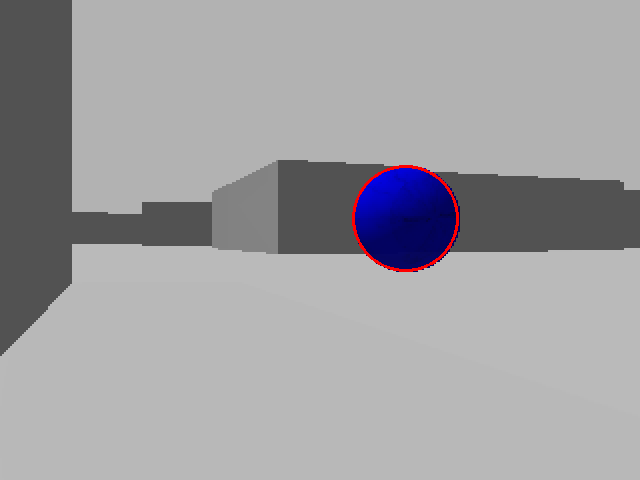
\includegraphics[width=\textwidth]{CV/camera_detected_marbles_2}
		\caption{Marble detection on scenario 1}
	\end{subfigure}
	\hfill
	\begin{subfigure}[b]{0.196\textwidth}
		\centering
		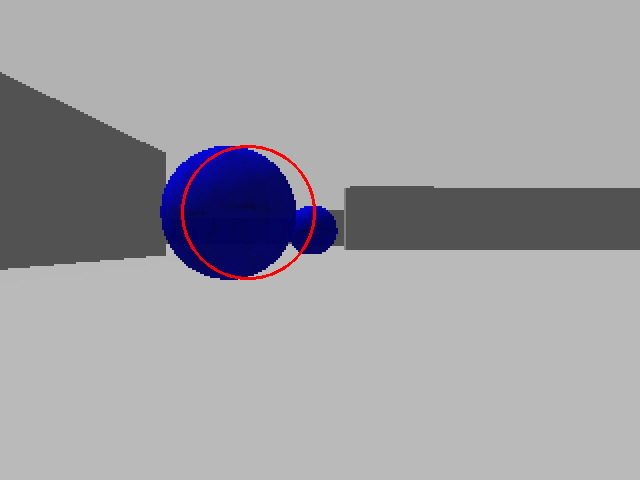
\includegraphics[width=\textwidth]{CV/camera_detected_marbles_3}
		\caption{Marble detection on scenario 2}
		\label{fig:md_2_impl}
	\end{subfigure}
	\hfill
	\begin{subfigure}[b]{0.196\textwidth}
		\centering
		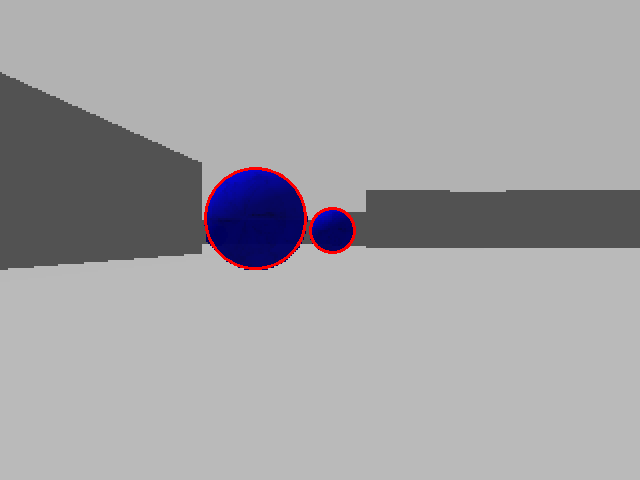
\includegraphics[width=\textwidth]{CV/camera_detected_marbles_4}
		\caption{Marble detection on scenario 3}
	\end{subfigure}
	\hfill
	\begin{subfigure}[b]{0.196\textwidth}
		\centering
		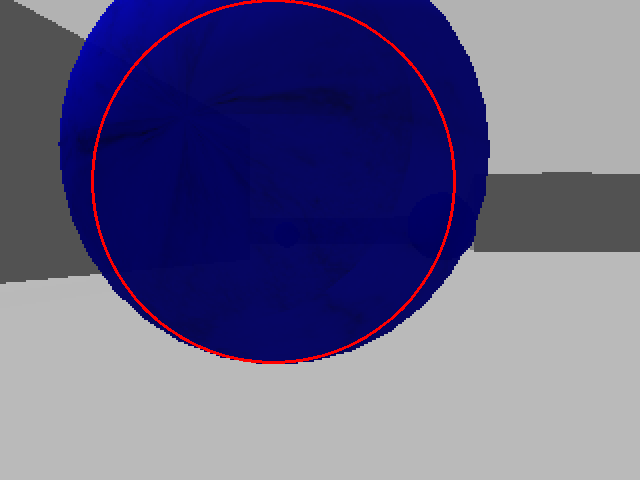
\includegraphics[width=\textwidth]{CV/camera_detected_marbles_5}
		\caption{Marble detection on scenario 4}
		\label{fig:md_4_impl}
	\end{subfigure}
	\hfill
	\begin{subfigure}[b]{0.196\textwidth}
		\centering
		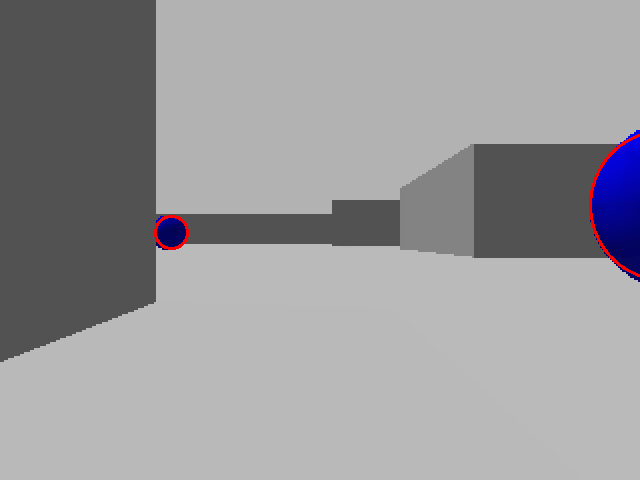
\includegraphics[width=\textwidth]{CV/camera_detected_marbles_6}
		\caption{Marble detection on scenario 5}
	\end{subfigure}
	\caption{Marble detection of scenario 1 to 5}
	\label{fig:md_1_5}
\end{figure} 
These issues was however not considered critical, because the one on figure (\ref{fig:md_4_impl}) will only occur when a marble is very close. The direction the robot needs to follow in order to collect the marbles would not be influenced by this error, only how close marble is.\\
The second issue, seen on figure (\ref{fig:md_2_impl}), could be a potential for the robot, due to the fact that the center of the marble are shifted. But as the robot moves closer the two marbles would either drift further apart enabling the algorithm to detect both, or the second marble found drift in behind the first one. 
\end{document}